\documentclass{standalone}
\usepackage{tikz}
\usetikzlibrary{patterns, positioning}

\begin{document}
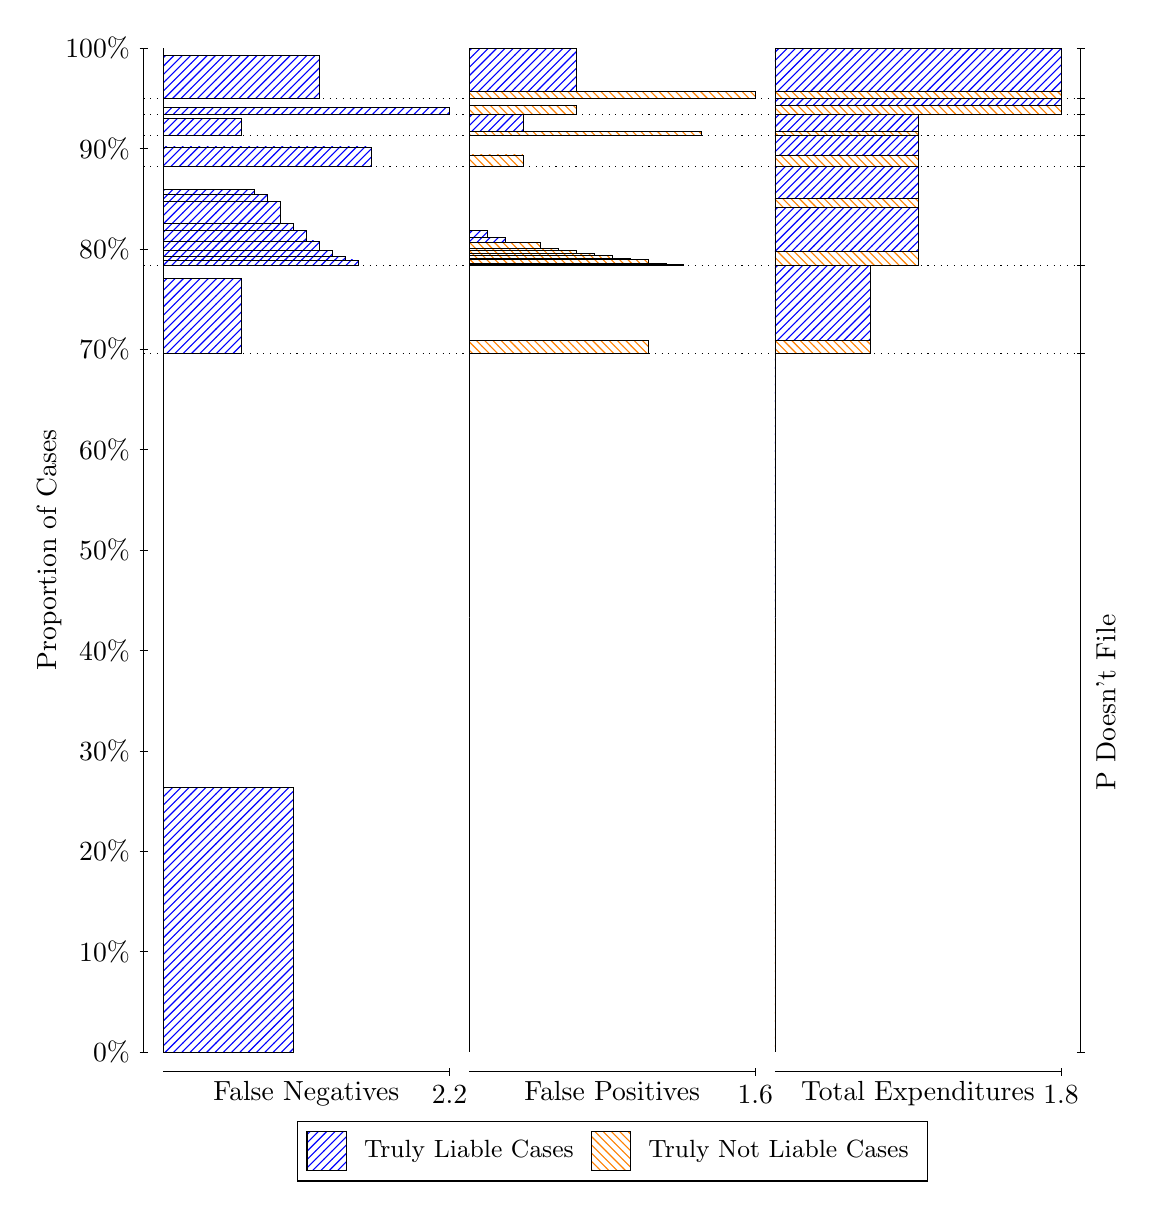
\begin{tikzpicture}
\draw[black, very thin] (1.5,1.75) -- (1.5,14.5);
\node[rotate=90, anchor=center] at (0.3, 8.125) {Proportion of Cases};
\draw[black, very thin] (1.45,1.75) -- (1.55,1.75);
\node[anchor=east] at (1.45, 1.75) {0\%};
\draw[black, very thin] (1.45,3.025) -- (1.55,3.025);
\node[anchor=east] at (1.45, 3.025) {10\%};
\draw[black, very thin] (1.45,4.3) -- (1.55,4.3);
\node[anchor=east] at (1.45, 4.3) {20\%};
\draw[black, very thin] (1.45,5.575) -- (1.55,5.575);
\node[anchor=east] at (1.45, 5.575) {30\%};
\draw[black, very thin] (1.45,6.85) -- (1.55,6.85);
\node[anchor=east] at (1.45, 6.85) {40\%};
\draw[black, very thin] (1.45,8.125) -- (1.55,8.125);
\node[anchor=east] at (1.45, 8.125) {50\%};
\draw[black, very thin] (1.45,9.4) -- (1.55,9.4);
\node[anchor=east] at (1.45, 9.4) {60\%};
\draw[black, very thin] (1.45,10.675) -- (1.55,10.675);
\node[anchor=east] at (1.45, 10.675) {70\%};
\draw[black, very thin] (1.45,11.95) -- (1.55,11.95);
\node[anchor=east] at (1.45, 11.95) {80\%};
\draw[black, very thin] (1.45,13.225) -- (1.55,13.225);
\node[anchor=east] at (1.45, 13.225) {90\%};
\draw[black, very thin] (1.45,14.5) -- (1.55,14.5);
\node[anchor=east] at (1.45, 14.5) {100\%};

\draw[black, very thin] (13.4,1.75) -- (13.4,14.5);
\draw[black, very thin] (13.35,1.75) -- (13.45,1.75);
\node[anchor=west] at (13.35, 1.75) {};
\draw[black, very thin] (13.35,10.625) -- (13.45,10.625);
\node[anchor=west] at (13.35, 10.625) {};
\draw[black, very thin] (13.35,11.743) -- (13.45,11.743);
\node[anchor=west] at (13.35, 11.743) {};
\draw[black, very thin] (13.35,12.995) -- (13.45,12.995);
\node[anchor=west] at (13.35, 12.995) {};
\draw[black, very thin] (13.35,13.392) -- (13.45,13.392);
\node[anchor=west] at (13.35, 13.392) {};
\draw[black, very thin] (13.35,13.655) -- (13.45,13.655);
\node[anchor=west] at (13.35, 13.655) {};
\draw[black, very thin] (13.35,13.862) -- (13.45,13.862);
\node[anchor=west] at (13.35, 13.862) {};
\draw[black, very thin] (13.35,14.5) -- (13.45,14.5);
\node[anchor=west] at (13.35, 14.5) {};

\draw[black, very thin, pattern color=blue, pattern=north east lines] (1.75,1.75) rectangle (3.4015,5.1088);
\draw[black, very thin, pattern color=orange, pattern=north west lines] (1.75,5.1088) rectangle (1.75,10.625);
\draw[black, very thin, pattern color=blue, pattern=north east lines] (1.75,10.625) rectangle (2.7409,11.577);
\draw[black, very thin, pattern color=orange, pattern=north west lines] (1.75,11.577) rectangle (1.75,11.743);
\draw[black, very thin, pattern color=blue, pattern=north east lines] (1.75,11.743) rectangle (4.2273,11.809);
\draw[black, very thin, pattern color=blue, pattern=north east lines] (1.75,11.809) rectangle (4.0621,11.853);
\draw[black, very thin, pattern color=blue, pattern=north east lines] (1.75,11.853) rectangle (3.897,11.934);
\draw[black, very thin, pattern color=blue, pattern=north east lines] (1.75,11.934) rectangle (3.7318,12.051);
\draw[black, very thin, pattern color=blue, pattern=north east lines] (1.75,12.051) rectangle (3.5667,12.185);
\draw[black, very thin, pattern color=blue, pattern=north east lines] (1.75,12.185) rectangle (3.4015,12.275);
\draw[black, very thin, pattern color=blue, pattern=north east lines] (1.75,12.275) rectangle (3.2364,12.553);
\draw[black, very thin, pattern color=blue, pattern=north east lines] (1.75,12.553) rectangle (3.0712,12.638);
\draw[black, very thin, pattern color=blue, pattern=north east lines] (1.75,12.638) rectangle (2.9061,12.706);
\draw[black, very thin, pattern color=orange, pattern=north west lines] (1.75,12.706) rectangle (1.75,12.995);
\draw[black, very thin, pattern color=blue, pattern=north east lines] (1.75,12.995) rectangle (4.3924,13.244);
\draw[black, very thin, pattern color=orange, pattern=north west lines] (1.75,13.244) rectangle (1.75,13.392);
\draw[black, very thin, pattern color=blue, pattern=north east lines] (1.75,13.392) rectangle (2.7409,13.609);
\draw[black, very thin, pattern color=orange, pattern=north west lines] (1.75,13.609) rectangle (1.75,13.655);
\draw[black, very thin, pattern color=blue, pattern=north east lines] (1.75,13.655) rectangle (5.3833,13.744);
\draw[black, very thin, pattern color=orange, pattern=north west lines] (1.75,13.744) rectangle (1.75,13.862);
\draw[black, very thin, pattern color=blue, pattern=north east lines] (1.75,13.862) rectangle (3.7318,14.409);
\draw[black, very thin, pattern color=orange, pattern=north west lines] (1.75,14.409) rectangle (1.75,14.5);
\draw[black, very thin, pattern color=orange, pattern=north west lines] (5.6333,1.75) rectangle (5.6333,7.2662);
\draw[black, very thin, pattern color=blue, pattern=north east lines] (5.6333,7.2662) rectangle (5.6333,10.625);
\draw[black, very thin, pattern color=orange, pattern=north west lines] (5.6333,10.625) rectangle (7.9042,10.791);
\draw[black, very thin, pattern color=blue, pattern=north east lines] (5.6333,10.791) rectangle (5.6333,11.743);
\draw[black, very thin, pattern color=orange, pattern=north west lines] (5.6333,11.743) rectangle (8.3583,11.753);
\draw[black, very thin, pattern color=orange, pattern=north west lines] (5.6333,11.753) rectangle (8.1313,11.766);
\draw[black, very thin, pattern color=orange, pattern=north west lines] (5.6333,11.766) rectangle (7.9042,11.811);
\draw[black, very thin, pattern color=orange, pattern=north west lines] (5.6333,11.811) rectangle (7.6771,11.832);
\draw[black, very thin, pattern color=orange, pattern=north west lines] (5.6333,11.832) rectangle (7.45,11.864);
\draw[black, very thin, pattern color=orange, pattern=north west lines] (5.6333,11.864) rectangle (7.2229,11.895);
\draw[black, very thin, pattern color=orange, pattern=north west lines] (5.6333,11.895) rectangle (6.9958,11.926);
\draw[black, very thin, pattern color=orange, pattern=north west lines] (5.6333,11.926) rectangle (6.7687,11.951);
\draw[black, very thin, pattern color=orange, pattern=north west lines] (5.6333,11.951) rectangle (6.5417,12.033);
\draw[black, very thin, pattern color=blue, pattern=north east lines] (5.6333,12.033) rectangle (6.0875,12.1);
\draw[black, very thin, pattern color=blue, pattern=north east lines] (5.6333,12.1) rectangle (5.8604,12.185);
\draw[black, very thin, pattern color=blue, pattern=north east lines] (5.6333,12.185) rectangle (5.6333,12.995);
\draw[black, very thin, pattern color=orange, pattern=north west lines] (5.6333,12.995) rectangle (6.3146,13.143);
\draw[black, very thin, pattern color=blue, pattern=north east lines] (5.6333,13.143) rectangle (5.6333,13.392);
\draw[black, very thin, pattern color=orange, pattern=north west lines] (5.6333,13.392) rectangle (8.5854,13.438);
\draw[black, very thin, pattern color=blue, pattern=north east lines] (5.6333,13.438) rectangle (6.3146,13.655);
\draw[black, very thin, pattern color=orange, pattern=north west lines] (5.6333,13.655) rectangle (6.9958,13.773);
\draw[black, very thin, pattern color=blue, pattern=north east lines] (5.6333,13.773) rectangle (5.6333,13.862);
\draw[black, very thin, pattern color=orange, pattern=north west lines] (5.6333,13.862) rectangle (9.2667,13.954);
\draw[black, very thin, pattern color=blue, pattern=north east lines] (5.6333,13.954) rectangle (6.9958,14.5);
\draw[black, very thin, pattern color=orange, pattern=north west lines] (9.5167,1.75) rectangle (9.5167,7.2662);
\draw[black, very thin, pattern color=blue, pattern=north east lines] (9.5167,7.2662) rectangle (9.5167,10.625);
\draw[black, very thin, pattern color=orange, pattern=north west lines] (9.5167,10.625) rectangle (10.728,10.791);
\draw[black, very thin, pattern color=blue, pattern=north east lines] (9.5167,10.791) rectangle (10.728,11.743);
\draw[black, very thin, pattern color=orange, pattern=north west lines] (9.5167,11.743) rectangle (11.333,11.915);
\draw[black, very thin, pattern color=blue, pattern=north east lines] (9.5167,11.915) rectangle (11.333,12.478);
\draw[black, very thin, pattern color=orange, pattern=north west lines] (9.5167,12.478) rectangle (11.333,12.595);
\draw[black, very thin, pattern color=blue, pattern=north east lines] (9.5167,12.595) rectangle (11.333,12.995);
\draw[black, very thin, pattern color=orange, pattern=north west lines] (9.5167,12.995) rectangle (11.333,13.143);
\draw[black, very thin, pattern color=blue, pattern=north east lines] (9.5167,13.143) rectangle (11.333,13.392);
\draw[black, very thin, pattern color=orange, pattern=north west lines] (9.5167,13.392) rectangle (11.333,13.438);
\draw[black, very thin, pattern color=blue, pattern=north east lines] (9.5167,13.438) rectangle (11.333,13.655);
\draw[black, very thin, pattern color=orange, pattern=north west lines] (9.5167,13.655) rectangle (13.15,13.773);
\draw[black, very thin, pattern color=blue, pattern=north east lines] (9.5167,13.773) rectangle (13.15,13.862);
\draw[black, very thin, pattern color=orange, pattern=north west lines] (9.5167,13.862) rectangle (13.15,13.954);
\draw[black, very thin, pattern color=blue, pattern=north east lines] (9.5167,13.954) rectangle (13.15,14.5);
\draw[black, dotted] (1.5,10.625) -- (13.4,10.625);
\draw[black, dotted] (1.5,11.743) -- (13.4,11.743);
\draw[black, dotted] (1.5,12.995) -- (13.4,12.995);
\draw[black, dotted] (1.5,13.392) -- (13.4,13.392);
\draw[black, dotted] (1.5,13.655) -- (13.4,13.655);
\draw[black, dotted] (1.5,13.862) -- (13.4,13.862);
\draw[black, very thin] (1.75,1.5) -- (5.3833,1.5);
\node[anchor=north] at (3.5667, 1.5) {False Negatives};
\draw[black, very thin] (5.3833,1.45) -- (5.3833,1.55);
\node[anchor=north] at (5.3833, 1.45) {2.2};

\draw[black, very thin] (5.6333,1.5) -- (9.2667,1.5);
\node[anchor=north] at (7.45, 1.5) {False Positives};
\draw[black, very thin] (9.2667,1.45) -- (9.2667,1.55);
\node[anchor=north] at (9.2667, 1.45) {1.6};

\draw[black, very thin] (9.5167,1.5) -- (13.15,1.5);
\node[anchor=north] at (11.333, 1.5) {Total Expenditures};
\draw[black, very thin] (13.15,1.45) -- (13.15,1.55);
\node[anchor=north] at (13.15, 1.45) {1.8};

\node[black, centered, rotate=90] at (13.72, 6.1875) {P Doesn't File};







\draw (7.449999999999999,1.5) node[draw=none] (baseCoordinate) {};
\begin{scope}[align=center]
        \matrix[scale=0.5, draw=black, below=0.5cm of baseCoordinate, nodes={draw}, column sep=0.1cm]{
            \node[rectangle, draw, minimum width=0.5cm, minimum height=0.5cm, pattern=north east lines, pattern color=blue] {}; &
            \node[draw=none, font=\small] (B) {Truly Liable Cases}; &
            \node[rectangle, draw, minimum width=0.5cm, minimum height=0.5cm, pattern=north west lines, pattern color=orange] {}; &
            \node[draw=none, font=\small] (B) {Truly Not Liable Cases}; \\
            };
\end{scope}

\end{tikzpicture}
\end{document}